\documentclass{article}
\usepackage{hyperref}
\usepackage{pdfpages}
\title{EMISY Project 21 Portable Compass}
\author{Krzysztof Rudnicki, 307585}
\date{\today}
\begin{document}
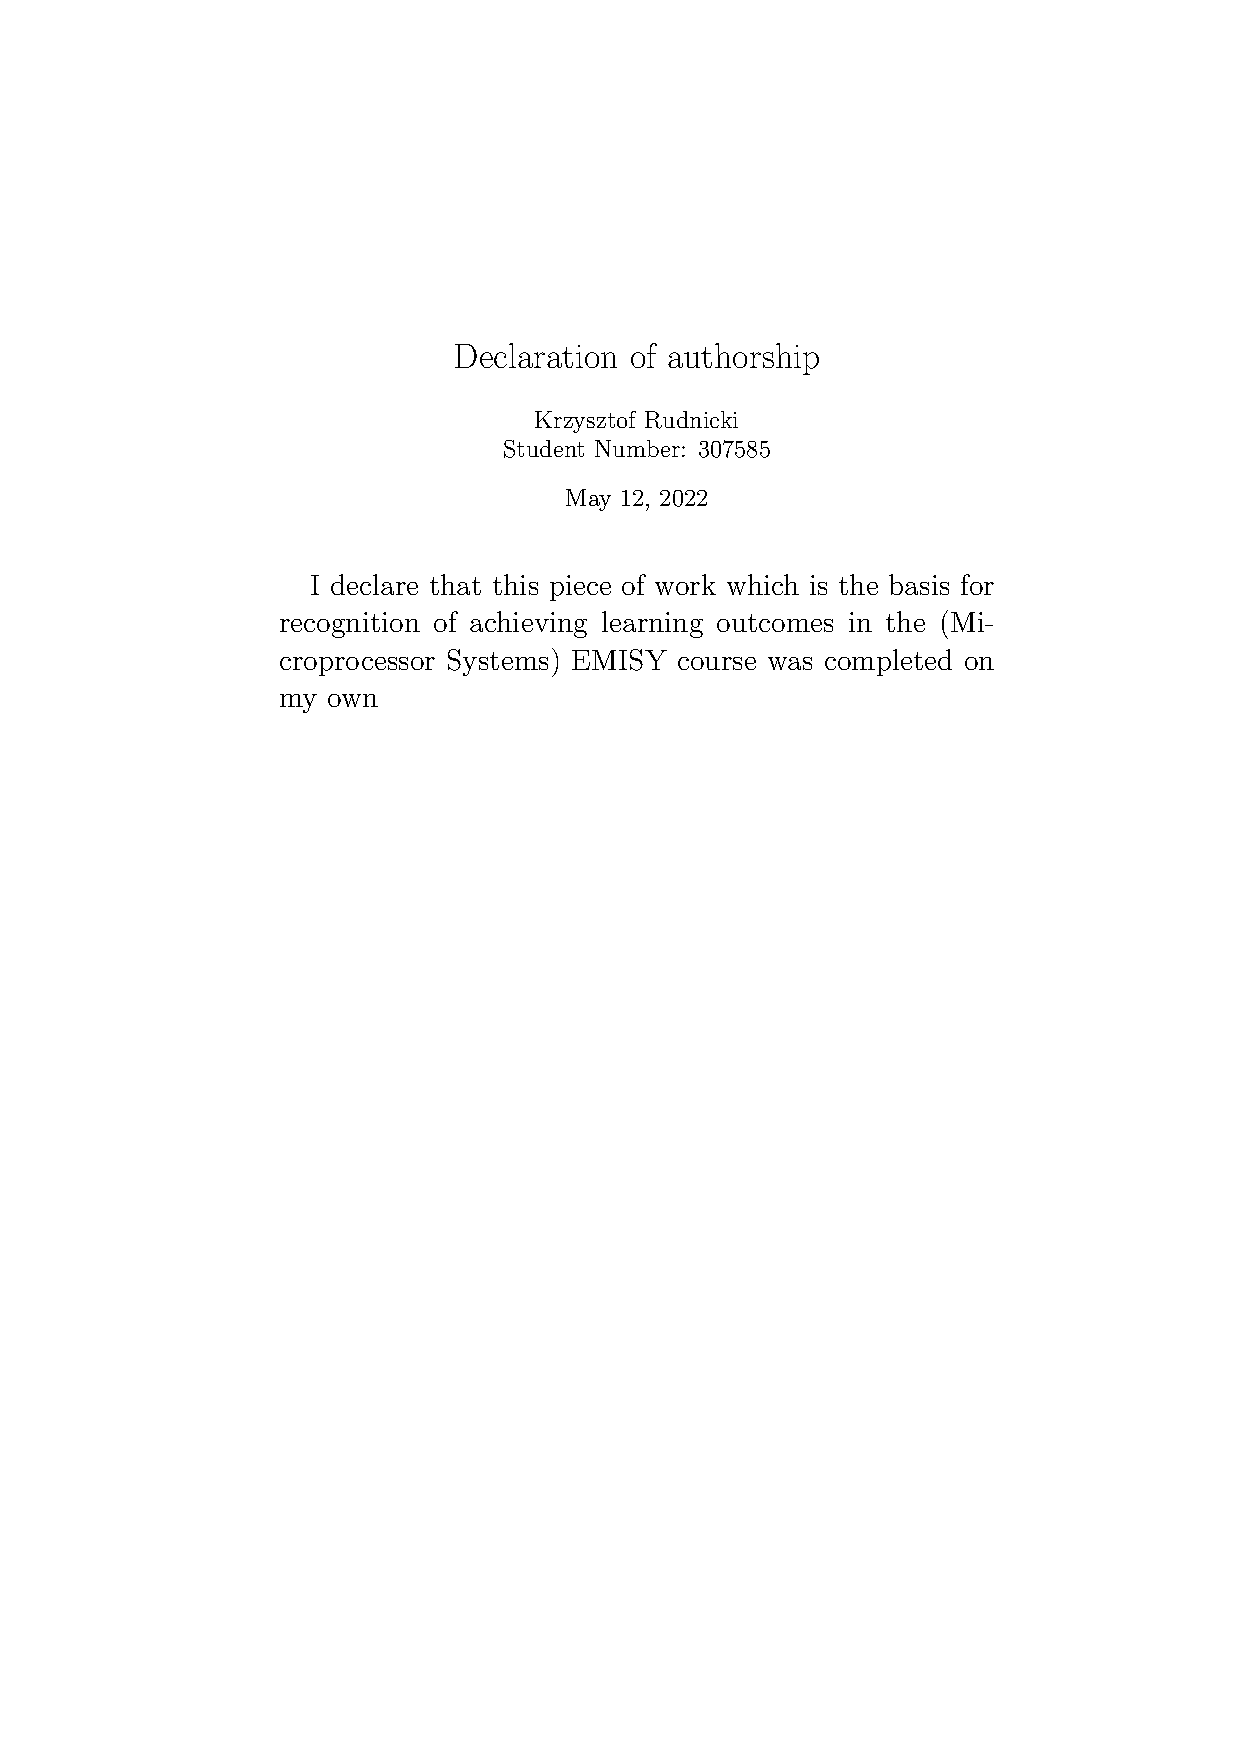
\includepdf[pages={1}]{declaration.pdf}
\maketitle
\section{Analysis of the project}
\subsection{Discussion of project requirements}
We need to create a simple portable compass circuit \\
It should:
\begin{itemize}
	\item Use energy-saving power modes of microcontroller
	\item Be battery powered
	\item Be portable (cellphone/wrist watch)
	\item Communicate using graphical OLED display and two buttons keyboard
\end{itemize}
\subsection{Discussion of solution}
\section{Detailed circuit diagram}
\section{Diagram}
\subsection{Diagram itself}
\subsection{Diagram description}
\subsubsection{How to make the project}
\subsubsection{Microcontroller}
I decided to use ATmega328P, 8-bit avr microcontroller.
\paragraph{Relatively small} Up to 9.25 mm $\times$ 9.25 mm dimensions, 
compared to apple watch display of 34 mm by 40 mm for smaller version. 
\cite{datasheet}
286th page
\paragraph{Square} It is shaped in a square which also simplifies portability
\cite{datasheet} 286th page
\paragraph{Popular} A lot of documentation, usecases, guides
\paragraph{5 software selectable power saving modes} Our device should use
energy-saving power modes and 5 is a plentiful choice \cite{datasheet} 7th
page
\\
Quick research suggests that this microcontroller can use as low as 0.36 mA
\cite{powerSavingModes}
\paragraph{Ease of use} In-system programming feature \cite{datasheet} (1 page)
and programming environments which allow for easy development of code.
\cite{avrgcc} 
\subsubsection{All other components}
\section{Draft of the microcontroller firmware}
\subsection{Block diagram}
\subsection{Description of the algorithm}
\begin{thebibliography}{9}
	\bibitem{datasheet} \href{https://ww1.microchip.com/downloads/en/DeviceDoc/Atmel-7810-Automotive-Microcontrollers-ATmega328P_Datasheet.pdf}{ATmega
	328P datasheet}
	\bibitem{powerSavingModes} \href{https://electronics.stackexchange.com/questions/49182/how-can-i-get-my-atmega328-to-run-for-a-year-on-batteries}{Electrical Engineering exchange,
	atmega328 one year on batteries}
	\bibitem{avrgcc} \href{https://gcc.gnu.org/wiki/avr-gcc}{avr gcc}
\end{thebibliography}
\end{document}
